\chapter{Implementácia programu}
V tejto kapitole sa budeme venovať niektorým významnejším črtám implementácie nášho programu, ktorý na vstupe dostane súbor popisujúci evolučnú históriu,
umožní používateľovi zmeniť niektoré nastavenia a prípadne spustiť optimalizáciu a nakoniec zobrazí grafickú reprezentáciu vstupnej evolučnej histórie podľa
toho, aké zmeny vykonal používateľ. Popíšeme v akom formáte má byť zapísaný vstup,
ako bude vyzerať výstup, aké kroky vykonajú triedy nášho programu,
akým spôsobom dokáže používateľ interagovať s programom,
ako nastavenia programu.
\section{Vstup}
\label{sec:vstup}

\begin{table}[!htb]
\label{tab:vstup}
\begin{center}
\begin{tabular}{llllllll}
predok & e1 & root & 0 & root & 1 2 1 5 4 3 2 & \#  & -1 -1 -1 -1 -1 -1 -1 \\
predok & e2 & e1 &  0.05 & dup &  1 2 1 2 5 4 3 2 & \# & 0 1 2 1 3 4 5 6 \\
clovek & e3 & e2 &  0.12 & sp &   1 2 1 2 5 4 3 2 & \# & 0 1 2 3 4 5 6 7 \\
clovek & e4 & e3 &  0.13 & del & 1 2 1 2 4 3 2 & \# & 0 1 2 3 5 6 7 \\
clovek & e5 & e4 &  0.14 & ins & 1 2 1 6 7 2 4 3 2 & \# & 0 1 2 -1 -1 3 4 5 6 \\
clovek &  e6 & e5 &  0.2 & inv &  1 -1 -2 6 7 2 4 3 2 & \# & 0 2 1 3 4 5 6 7 8 \\
clovek & e7 & e6 &  0.25 & leaf & 1 -1 -2 6 7 2 4 3 2 & \# & 0 1 2 3 4 5 6 7 8 \\
simpanz & e8 & e2  & 0.12 & sp &  1 2 1 2 5 4 3 2 & \# & 0 1 2 3 4 5 6 7 \\
simpanz & e9 & e8 &  0.2 & leaf & 1 2 1 2 5 4 3 2 & \# & 0 1 2 3 4 5 6 7 \\
 \end{tabular}

\end{center}
\caption{Ukážka vymysleného vstupu v súčasnom formáte.}
\end{table}

Vstupom do nášho programu je evolučná história, ktorá popisuje poradie génov v jednotlivých krokoch, a aké
sú vzťahy medzi génmi v nasledujúcich krokoch histórie.
Vstupný súbor nášho programu bude tvoriť postupnosťou riadkov, podobná tej akú vidíme v tabuľke  \ref{tab:vstup}.
Každý riadok predstavuje jeden \emph{krok evolučnej histórie}.
Prvý riadok je koreňom danej histórie, opisuje prvotný stav sekvencie a má priradenú 
špeciálnu udalosť "root".
Každý ďalší riadok opisuje niektorý z nasledujúcich krokov histórie. 
Riadok obsahuje zoznam génov nachádzajúcich sa v tomto kroku
a spolu so svojím predchodcom nám umožňuje určiť aké evolučné udalosti viedli k súčasnému stavu.
Predchodca sa v súbore musí nachádzať vždy skôr než nasledovník, aj preto je prvým riadkom koreň.
Riadok obsahuje niekoľko reťazcov a čísel, oddelených medzerou alebo viacerými medzerami, ak je to potrebné pre lepšiu prehľadnosť.
\paragraph{Význam stĺpcov:}

\begin{description}

\item[Prvý stĺpec] je názov biologického druhu (súčasného alebo určitého predka),
ktorého sa týka daný riadok.

\item[Druhý stĺpec] je id riadku.

\item[Tretí stĺpec] je id predchodcu, t.j. kroku histórie ktorý nastal bezprostredne pred aktuálnym krokom.
Prvý riadok má špeciálne id predchodcu s hodnotou ''root'. Hoci každý riadok okrem koreňa má jednoznačného predka, naopak to neplatí.
V príklade vyššie má riadok $e2$ dvoch potomkov, 
to znamená že v tomto kroku histórie nastala speciácia a vznikol nový druh, riadok $e7$ nemá žiadneho potomka, 
tento krok je ukončením jednej vetvy evolučnej histórie.

\item[Štvrtý stĺpec] je čas, v ktorom sa daná udalosť odohrala. Koreň sa nachádza v čase 0, a čas smerom k súčasnosti rastie.

\item[Piaty stĺpec] je skratka niektorej z udalostí, popísaných v sekcii \ref{evhist}, pokiaľ sa v danom kroku evolučnej histórie odohrala iba jedna z týchto udalostí, alebo jedna zo trojice udalostí root/leaf/other.
Root je udalosť slúžiaca na identifikáciu koreňa.
Leaf slúži na určenie času, v ktorom sa daná vetva končí, medzi udalosťou označenou ako leaf a jej predchodcom nemuselo prísť k žiadnym zmenám.
Other použijeme, ak rozdiely medzi týmto a predchádzajúcim krokom nie sme schopní popísať pomocou jednej udalosti.
Znamená to, že takýto krok vznikol kombináciou viacerých udalostí ako napríklad dve duplikácie nasledujúce po sebe alebo translokácia s následnou deléciou.

\item [Nasledujúce stĺpce] obsahujú postupnosť génov v poradí, v akom sa nachádzajú v chromozóme.
Identifikátorom každého génu je celé číslo, pričom znamienko určuje jeho orientáciu. 
To znamená že gén 2 je rovnaký ako gén -2, iba opačne orientovaný v rámci DNA.

\item [Znak \#] slúži ako ukončenie zoznamu génov.

\item[Zvyšné stĺpce] pre každý gén určujú poradie predka génu v predchodcovi jeho riadku. Ak tento gén nemá predchodcu, obsahuje riadok hodnotu -1.
Napríklad pre druhý výskyt génu 2 v riadku e4 vieme, že poradie jeho predchodcu má index 3. Keďže predchodcom e4 je e3 vieme spojiť štvrtý (indexujeme od nuly) gén z riadku e3 s štvrtým génom (gén 2) riadku e4.

\end{description}

\section{Návrh výstupu}
\label{sec:vykreslene}
Naším cieľom je zobraziť 
kompletnú informáciu o génoch, ktoré sa nachádzajú v evolučnej histórii.
Potrebujeme preto nájsť spôsob ako túto informáciu pridať do fylogenetického stromu.
Naše zobrazenie evolučnej histórie bude predstavovať
les stromov, v ktorom jednotlivé stromy reprezentujú gény nachádzajúce sa v skúmaných druhoch. 
Každý gén bude zobrazený počas celej jeho existencie v evolučnej histórii. 
Os $x$ slúži ako os času, naľavo sa nachádza čas 0, ktorý postupne rastie tak, aby sa do obrázku zmestil aj najneskorší krok evolučnej histórie.

\emph{Gény} sú znázornené farebnými čiarami, ktoré idú vodorovne, až kým sa nedostanú do bodu, v ktorom má nastať udalosť.
Ak sa nasledujúci krok $k$ evolučnej histórie nachádza v čase $t_k$, tak gény dojdú bez zmeny do bodu $t_k - d$,
kde $d$ reprezentuje čas potrebný pre zobrazenie zmien. Zmeny vedúce ku kroku $k$ sa teda udejú počas časového rozmedzia $t_k - d$ až $t_k$.
Pozícia génov v rámci osi $y$ je v udalosti root daná ich reálnym poradím, pričom prvý gén sa nachádza najvyššie.
Pre každý ďalší krok tiež platí, že gény daného kroku sú na osi $y$ zoradené podľa poradia, v akom sa nachádzajú v tomto kroku evolučnej histórie.

Duplikáciu, teda skopírovanie jedného alebo viacerých génov, zobrazíme tak, že každý zo stromov reprezentujúci zduplikované gény rozvetvíme. 
Vetvenie začne v čase $t_k - d$.

Speciáciu by sme v klasickom druhovom fylogenetickom strome zobrazili ako rozvetvenie druhového stromu,
počas speciácie teda rozvetvíme všetky gény
- získame dve sady vetiev reprezentujúce naše gény v dvoch dcérskych organizmoch.
Rozdiel medzi speciáciou a duplikáciou všetkých génov je zreteľný vo vzdialenosti na osi $y$,
kedy pri speciácii rozoznávame dve sady vetiev, ktoré sú od seba dostatočne vzdialené,
zatiaľ čo duplikácia by nechala všetky nové gény spolu. Ak sa jedna vetva speciácie nachádza v čase $t_a$ a druhá v čase $t_b$, zobrazíme 
začiatok speciácie do času $t_x - d$ kde $t_x$ je skorší z časov $t_a,t_a$.

Inzerciu génov znázorníme pridaním nového stromu pre každý vložený gén, začiatok pridaných stromov sa nachádza v čase $t_k$.
Deléciu génu zobrazíme ako ukončenie vetvy stromu, ktorá reprezentovala inštanciu tohto génu, takúto vetvu ukočíme v čase $t_k - d$.

Transpozíciu zobrazíme ako kríženie vetiev transponovaných génov tak, aby sa po tomto krížení nachádzali vetvy v správnom poradí,
kríženie sa začne v čase $t_k - d$ a skončí v čase $t_k$.

Inverziu znázorníme podobne ako transpozíciu, avšak keďže pri inverzii okrem zmeny poradia génov dochádza aj k zmene ich orientácie, pridáme do zobrazenia údaj o orientácii génu.
Gén so zmenenou orientáciou nebudeme zobrazovať plnou čiarou ale prerušovanou. To nám umožní zobraziť inverziu jedného génu,
ktorá by inak nemusela byť viditeľná a inverziu dvoch génov, ktorú by sme si mohli pomýliť s transpozíciou. 
Zmena štýlu čiary nastáva už v čase  $t_k - d$.

Root je začiatok pre všetky stromy génov, ktoré sa nachádzajú v počiatočnom predkovi.
Leaf ukončí vetvy génov v čase $t_k$.

 
Obrázok \ref{obr:events} ilustruje všetky udalosti, ktoré sme práve opísali.
Naľavo sa nachádza krok evolučnej histórie ''root'' obsahujúci štyri gény,
nasleduje inzercia dvoch ďalších génov a po nej speciácia.
Pri speciácii vzniknú dve vetvy génov ktoré sú od seba dostatočne vzdialené na to aby sme ich rozoznali.
Navyše vrchná vetva speciácie sa začína v neskoršom čase, nachádza sa v nej duplikácia dvoch génov a ukončenie v liste.
V spodnej vetve sa odohráva inverzia, po nej transpozícia a nakoniec delécia dvoch génov a ukončenie zvyšných v liste.

\begin{figure}
\centerline{\includegraphics[width=1\textwidth]{images/udalosti}}
\caption{Príklad zobrazenia histórie naším programom}\label{obr:events}
\end{figure}

\section{Triedy programu EHDraw}
V stručnosti si predstavíme základne funkcie, ktoré plnia triedy v našom programe.
\paragraph{EHDraw} je hlavnou triedou nášho programu.
Načíta vstupné parametre, a na ich záklde sa rozhodne či program prebehne neinteraktívne, iba na základe prvotného vstupu, 
alebo sa spustí interaktívna grafická aplikácia využívajúca JavaFX, ktorá je zapísaná v tejto triede.
\paragraph{EvolutionTree} je kľúčovou triedou celého projektu, reprezentuje evolučnú históriu,
obsahuje výpočty potrebné pre jej vykreslenie ako aj optimalizáciu.
Obsahuje podtriedu \emph{EvolutionNode},
ktorá popisuje jeden krok evolučnej histórie. Táto trieda dostane vstupnú históriu a tú si uloží vo vhodných dátových štruktúrach.
Pre každý krok evolučnej histórie si vytvorí jeden \emph{EvolutionNode} v ktorom okrem referencie predchodcu, drží aj referencie na jeho nasledovníka alebo nasledovníkov, pokiaľ nejakých má.
V triede \emph{EvolutionTree} si zapamätáme \emph{EvolutionNode} pre krok root, a ku všetkým zvyšným \emph{EvolutionNode} sa z neho dostaneme rekurzívne. 


Pri vykresľovaní zisťuje, akú šírku bude krok zaberať na obrázku. Pre list je táto šírka daná súčtom šírok jeho génov a medzier medzi nimi. 
Pre zvyšné kroky je daná buď ako ich vlastná šírka, to znamená výpočet rovnaký ako pri liste,
alebo ako šírka kroku, ktorý po ňom nasleduje.
Vyberáme väčšiu z týchto dvoch hodnôt.
Pokiaľ v kroku nastáva vetvenie druhového stromu, vyberieme ako jeho šírku väčšiu z hodnôt
jeho vlastnej šírky, alebo súčtu šírok krokov, ktoré z neho vychádzajú, a medzery, ktorú medzi nimi musíme nechať.
Keď poznáme šírky, ktoré potrebujú jednotlivé kroky, môže vykresliť našu evolučnú históriu.

V tejto triede taktiež prebieha aj výber génov na zobrazenie, ktorý bližšie popíšeme v časti \ref{blok}.



\paragraph{DrawFactory} je abstraktná trieda slúžiaca pre vykresľovanie evolučnej histórie.
V našom programe sa nachádzajú dve triedy, ktoré ju rozširujú.
\emph{FXDrawFactory} slúži na vykreslenie evolučnej histórie v našej JavaFX aplikácii. 
\emph{SVGDrawFactory} slúži na vykreslenie evolučnej histórie vo formáte \emph{svg} - škálovateľná vektorová grafika,
využíva k tomu knižnicu \emph{Apache Batik}.
Históriu v tomto formáte vieme následne vyexportovať do súboru. Export je funkcionalita ktorú ponúka iba \emph{SVGDrawFactory}.
\emph{EvolutionTree} dostane inštanciu jednej z týchto dvoch tried a pomocou nej vykreslí evolučnú históriu.
\paragraph{GeneMeta} reprezentuje nastavenia jedného génu, spôsob ako ich exportovať do XML
a tiež možnosť načítať takéto nastavenia z XML súboru.
\paragraph{Settings} V tejto triede sa nachádzajú globálne nastavenia ktoré využívame
pre vykresľovanie. Sú tu uložené aj \emph{GeneMeta} pre niektoré gény.
pokiaľ pre gén neexistuje \emph{GeneMeta}, alebo neobsahujú hodnotu pre požadované nastavenie, 
využije sa všeobecná hodnota tohto nastavenia, ktorá sa nachádza v triede \emph{Settings}.
Trieda \emph{Settings} taktiež obsahuje možnosť vyexportovať nastavenia, vrátane vrátane všetkých 
\emph{GeneMeta}, do XML súboru, ako aj možnosť nastavenia z XML súboru načítať.

\section{Ovládanie programu}
Náš program ponúka dve možnosti ako ho ovládať. Prvou z nich je grafická aplikácia ktorá používateľovi 
umožňuje interagovať s nastaveniami a 
spúšťať funkcie ktoré program obsahuje.
Druhou možnosťou je vložiť programu všetky požiadavky, ktoré má splniť v príkazovom riadku
už pri jeho spustení, tento spôsob nevyžaduje žiadnu ďalšiu interakciu a je ideálny pri potrebe
spracovať väčšie množstvo vstupov.
Teraz sa pozrieme na to aké možnosti ovládania tieto dve alternatívy ponúkajú.
\subsection{Grafická aplikácia}
\begin{figure}[t]
 \centering
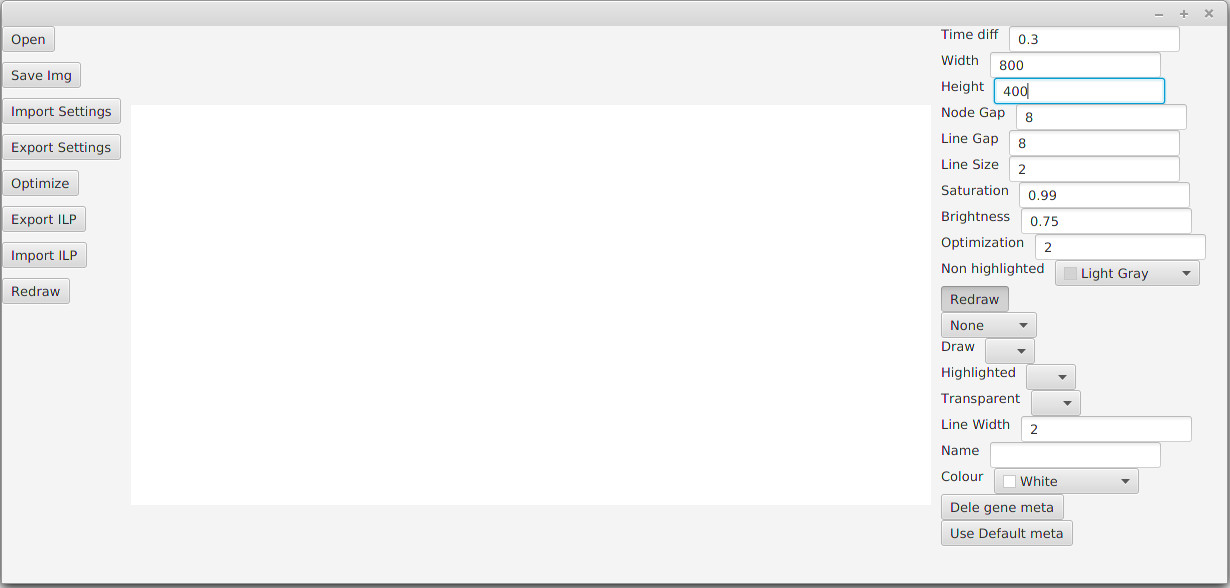
\includegraphics[width=1\textwidth]{images/gui}
\caption{Vzhľad grafickej aplikácie}\label{obr:gui}
\end{figure}

Na obrázku \ref{obr:gui} vidíme základné okno našej aplikácie. V strede sa nachádza plocha na ktorú sa 
vykresľuje evolučná história. Na ľavo sa nachádza sada tlačidiel a na pravo ovládacie prvky pre zmenu nastavení.
Pri spustení má aplikácia rozmery 1200x800 a plocha, na ktorú sa vykresľuje rozmery 800x800.
\paragraph{Tlačidlá na ľavej strane} slúžia k základnému ovládaniu nášho programu, popíšeme čo ktoré tlačidlo po stlačení vykoná,
a aké to má využitie.

\emph{Open} otvorí nové okno ktoré nám umožní zvoliť súbor, ktorý chceme otvoriť, tento súbor by mal byť vo formáte popísanom v sekcii \ref{sec:vstup}. 
 Zvolená evolučná história sa načíta a vykreslí. 
 
\emph{Save Img} otvorí nové okno, ktoré nám umožní zvoliť si do akého súboru sa uloží náš súčasný obrázok, ten sa ukladá vo formáte SVG.

\emph{Import Settings} v novom okne nám umožní vybrať si súbor vo formáte XML obsahujúci nastavenia, ktoré má načítať.

\emph{Export Settings} umožňuje vybrať súbor do ktorého sa uložia naše nastavenia. Nastavenia sa ukladajú vo formáte XML.

\emph{Optimize} zostrojí problém množinového pokrytia tak ako je to popísané v kapitole \ref{chap:setcover}
a následne nájde jeho približné riešenie pomocou greedy algoritmu.
Podla toho akú hodnotu má pole \emph{optimization} sa toto riešenie prenesie do zobrazenia.

\emph{Export ILP} podobne ako tlačidlo \emph{Optimize} zostrojí problém množinového pokrytia, 
a ten uloží zapísaný ako celočíselný lineárny program, do nami zvoleného súboru.

\emph{Import ILP} v novom oknem nám umožní zvoliť súbor, ktorý sa otvorí, tento súbor obsahouje riešenia celočíselného lineárneho programu.
 Náš program je nastavený tak aby vedel spracovať riešenia ktoré produkuje \emph{CPLEX}, to akým spôsobom sa načítané riešenie prenesie do 
 zobrazenia evolučnej histórie, závisí od toho, aká hodnota sa nachádza v poli \emph{optimization}.
 
\emph{Redraw} po stlačení tohto tlačidla dôjde k prekresleniu obrázku.
\paragraph{Ovládacie prvky na pravej strane}
Na pravej strane sa nachádzajú dve sady ovládacích prvkov. Prvá sada mení nastavenia ktoré sa 
nachádzajú priamo v triede \emph{Settings} a sú zdielané všetkými génmi a celým prostredím.
Druhá sada mení nastavenia špecificky pre zvolený gén, je to teda spôsob akým meníme nastavenia triedy
\emph{GeneMeta} pre konkrétny gén.
\paragraph{Globálne}\mbox{}\linebreak
\emph{Time diff}je číslo vyjadrujúce koľko času má zabrať zobrazenie udalosti na X-ovej osi, 
ak má krok evolučnej histórie $k$ známy čas $t_k$ tak 
jeho udalosť sa začne odohrávať už v čase $t_k - \emph{Time diff}$, tento čas však nesmie byť menší ako čas
v ktorom sa odohral predchodca kroku $k$. Time diff reprezentuje rovnakú premennú ako znak $d$ v sekcii 
\ref{sec:vykreslene}. 

\emph{Width} určuje dĺžku osi $x$, teda šírku obrázku, náš program každú evolučnú históriu naškáluje tak, aby ležala na celej tejto osi.
Zadáva sa celé číslo.

\emph{Height} určuje dĺžku osi $y$, teda výšku obrázku, náš program na šírku neškáluje, to aká časť šírky je pokrytá závisí od šírok génov a ich medzier.
Zadáva sa celé číslo.

\emph{Node Gap} určuje vzdialenosť medzi dvoma sadami vetiev, ktoré vznikli počas speciáce.
Zadáva sa celé číslo.

\emph{Line Gap} určuje medzeru medzi dvoma susednými génmi, ktoré sa nachádzajú v jednom kroku evolučnej histórie.Zadáva sa celé číslo.

\emph{Line Size} šírka čiary jedného génu, platí pre všetky gény, pokiaľ nemajú svoje vlastné špecifické nastavenie.Zadáva sa celé číslo.

\emph{Saturation} a \emph{Brightness} nastavenie sýtosti a jasu farieb.
Farby génom priraďujeme z modelu HSB - hue,saturation,brightness - slovensky odtieň,sýtosť,jas.
Odtieň v tomto modeli je daný v stupňoch hodnotou $0^\circ-360^\circ$. To nám umožňuje rovnomerne rozdeliť odtiene medzi $n$ génov.
Sýtosť a jas sú potom pre všetky gény rovnaké, určujeme ich reálnym číslo z rozmedzia $<0,1>$ . 


\emph{Optimization} určuje akým spôsob sa prejaví optimalizácia na výslednom zobrazení evolučnej histórie.
Pri hodnote 2 sa génom, ktoré sa nenachádzajú v riešení nastaví atribút $higlighted=false$, vykreslia sa farbou ktorá je daná ako
\emph{Non highlighted}, takéto nastavenie vidíme na obrázku \cite{obr:opt} v okienku číslo 2.
Pri hodnote 1 sa nezvolením génom nastaví atribút $trasnparent=true$, zobrazia sa priesvitne, rovnako ako v okienku číslo 3.
Pri hodnote 0 sa nezvolením génom nastaví atribút $draw=false$, a teda sa nezobrazia vôbec, rovnako ako štvrtom okienku.

\emph{Non highlighted} umožňuje výber farby pre gény, ktoré nie sú zvýraznené.
To sú tie pre ktoré $highlighted=false$ a zároveň $draw=true$ a $transparent=false$. Tieto hodnoty génom manuálne nastavíme
alebo ich získajú pokiaľ sa nenachádzajú v riešení optimalizácie a $optimization=2$.

\emph{Redraw} je prepínač, pokiaľ je zapnutý, obrázok sa automaticky prekreslí po tom, čo zmeníme niektoré z jeho nastavení. 
V opačnom prípade obrázok prekreslíme stlačením ľavého tlačidla \emph{Redraw}.
\paragraph{Špecifické pre gén} sa aplikujú na vybraný gén ktorý zvolíme zo zoznamu.
V tomto zozname sa nachádzajú všetky gény z histórie, bez ohľadu na to, či pre ne existuje záznam \emph{GeneMeta} uložení v nastaveniach
\emph{Settings}.
Okrem toho sa v liste nachádzajú dve špeciálne hodnoty. \emph{None} vyjadruje že nemáme zvolený žiaden gén a nebudeme vedieť meniť žiadne 
nastavenia špecifické pre gén. \emph{Default} slúži k nastaveniu hodnôt, ktoré využívajú všetky gény bez vlastných \emph{GeneMeta}.
Pre \emph{Default} nevieme nastavovať \emph{Name} ani \emph{Colour}.
Pokiaľ si z listu zvolíme gén ktorý nemá vlastný záznam \emph{GeneMeta}, tento záznam sa vytvorí až keď tomuto génu nastavíme niektorú z
hodnôt.Do polí \emph{Draw,Transparent a Highlighted} sa prekopíruje hodnota nastavená v \emph{Default}, zvyšné polia môžu zostať prázdne.
Pre prázdne polia sa aj naďalej využívajú hodnoty z \emph{Default}.

\emph{Draw} boolean prepínač, hodnota určuje či sa gén vykreslí.

\emph{Transparent} boolean prepínač, pokiaľ sa má gén vykresliť $(draw=true)$, tak hodnota \emph{Transparent} určí, či bude priesvitný $transparent=true$, kedy gén nevidíme, ale zaberá miesto.
Alebo bude nepriesvitný, kedy farbu získa v závislosti od hodnoty \emph{Highlighted}.

\emph{Highlighted} pokiaľ sa má gén nepriesvitne vykresliť $draw=true,transparent=false$ highlighted rozhodujem o tom, či bude zvýraznený.
Ak je zvýraznený zobrazí sa s farbou ktorú má nastavenú v \emph{Colour}, v prípade že nemá nastavenú vlastnú farbou použije predpočítanú farbu.
Ak nieje zvýraznený použije farbu nastavenú v \emph{Non Highlighted}. 

\emph{Line Width} umožňuje individuálne nastavenie šírky génu. Vkladáme celé číslo.

\emph{Name} je textové pole, v ktorom môžme génu nastaviť jeho meno.

\emph{Colour} ponúka výber farby špeciálne pre daný gén.

\emph{Delete gene meta} odstráni záznam \emph{GeneMeta} pre práve zvolený gén.Nefunguje pre \emph{Default}.

\emph{Delete all meta} odstráni všetky existujúce záznamy \emph{GeneMeta} okrem záznamu \emph{Default}.

\subsection{Argumenty príkazového riadku}
Nie vždy pre nás musí byť výhodnejšie, ovládať náš program cez grafickú aplikáciu. 
Ako alternatívu ku grafickej aplikácii ponúka náš program možnost, vložiť mu základné parametre potrebné pre jeho beh už pri jeho spustení.
Program potom sám vykoná zvolené úkony, bez potreby akejkoľvek ďalšej interakcie zo strany uživateľa. 
Tento spôsob ovládania programu je výhodný napríklad vtedy, keď cheme automatizovať spracovanie väčšieho počtu vstupov.
Predstavíme si aké argumenty vieme vložiťna príkazový riadok, a aký vplyv budú mať na priebeh nášho programu. 
Každý argument ktorý týtmto spôsobom programu vložíme má na začiatku pomlčku. Poradie argumentov nie je dôležité.

\emph{-nogui} argument určujúci že náš program nespustí grafickú aplikáciu, ale vystačí si len s údajmi zo vstupu.

\emph{-input:filename.history} argument, ktorým ukážeme na súbor "filename.history"\ obsahujúci evolučnú históriu.
Evolučná história ktorá sa nachádza v tomto súboré sa načíta do programu.

\emph{-drawsvg} nahraná evolučná história sa vykreslí vo formáte svg do súboru output.svg.

\emph{-svg\_output:filename.svg} miesto súboru output.svg sa obrázok uloží do súboru "filename.svg".

\emph{-opt:x} prebehne optimalizáciu počtu zobrazených génov, číslo x má rovnakú funkciu ako nastavenie \emph{Optimization} z grafickej aplikácie.

\emph{-exportgreedy} do súboru output.greedy uloží greedy riešenie problému množinového pokrytia pre nahranú evolučnú históriu.

\emph{-greedy\_output:filename.svg} miesto do súboru output.greedy sa greedy riešenie uloží do súboru "filename.svg".

\emph{-exportilp} zadanie celočíselného lineárneho programu - \ref{sub:bclp},
ktorý je ekvivalentný k problému množinového pokrytia pre nahranú evolučnú históriu, sa uloží do súboru output.lp

\emph{ilp\_output:filename.lp} namiesto output.lp sa pre uloženie zadanie celočíselného lineárneho programu využije súbor "filename.lp".

\emph{-load\_lp:input.sol} optimalizuje zobrazené gény na základe riešenia zo súboru ''input.sol".
Program je nastavený tak aby akceptoval riešenie ktoré prodkuje CPLEX.

\emph{-load\_settings:filename.xml} do triedy \emph{Settings} načítana nastavenia zo súboru ``filename.xml''.

